% -*- TeX-engine: luatex -*-
\documentclass[presentation,aspectratio=43,10pt]{beamer}
\usepackage{pgfplots}
\usepackage{template}
\renewcommand{\authorname}{Lawrence Mitchell\inst{*}}
\renewcommand{\authoremail}{\inst{*}\texttt{lawrence.mitchell@durham.ac.uk}}

\renewcommand{\sessionnumber}{3}
\renewcommand{\sessiontitle}{Roofline models}
\usepackage{tikz}
\usetikzlibrary{matrix,fit,positioning,calc}
\usepackage{pgfplotstable}
\pgfplotsset{compat=1.17}
\usetikzlibrary{pgfplots.groupplots}
\date{}

\begin{document}
\begin{frame}
  \maketitle
\end{frame}

\begin{frame}
  \frametitle{Parallel load bandwidth}
  In exercise 3, you hopefully produced plots similar to these.
  \begin{center}
    \begin{tikzpicture}
      \begin{groupplot}[
        group style={
          group size=2 by 2,
          ylabels at=edge left,
          vertical sep=15,
        },
        width=0.5\textwidth,
        height=0.5\textheight,
        ytick align=outside,
        xtick align=outside,
        enlarge x limits=false]
        \pgfplotstableread[col sep=comma, row sep=\\]{
Cores,MBytes\\
1,235851.41\\
2,496877.99\\
3,710912.58\\
4,921641.13\\
5,1119651.07\\
6,1340244.96\\
7,1567297.31\\
8,1791117.77\\
9,2009568.60\\
10,2233087.23\\
11,2460103.88\\
12,2686223.11\\
}\lonepacked
\pgfplotstableread[col sep=comma, row sep=\\]{
Cores,MBytes\\
2,499352.31  \\
4,997948.66  \\
6,1415179.90 \\
8,1835389.17 \\
10,2230741.49\\
12,2683507.01\\
14,3122751.55\\
16,3568497.34\\
18,4014922.79\\
20,4460070.15\\
22,4917133.09\\
24,5350956.73\\
}\lonespread
\pgfplotstableread[col sep=comma, row sep=\\]{
Cores,MBytes\\
1,78953.00  \\
2,145816.61 \\
3,204072.37 \\
4,268238.93 \\
5,327294.56 \\
6,390499.89 \\
7,353538.14 \\
8,412698.19 \\
9,587899.76 \\
10,656559.26\\
11,562220.33\\
12,595727.88\\
}\ltwopacked
\pgfplotstableread[col sep=comma, row sep=\\]{
Cores,MBytes\\
2,137955.69  \\
4,289802.29  \\
6,410549.79  \\
8,537170.25  \\
10,656448.64 \\
12,594029.39 \\
14,692981.85 \\
16,820538.24 \\
18,886785.12 \\
20,973679.48 \\
22,1264000.99\\
24,1189243.72\\
}\ltwospread
\pgfplotstableread[col sep=comma, row sep=\\]{
Cores,MBytes\\
1,36802.52  \\
2,64944.71  \\
3,96418.87  \\
4,121832.13 \\
5,149241.06 \\
6,174534.94 \\
7,210164.67 \\
8,239854.36 \\
9,267495.01 \\
10,295282.00\\
11,321351.58\\
12,353565.40\\
}\lthreepacked
\pgfplotstableread[col sep=comma, row sep=\\]{
Cores,MBytes\\
2,66484.66  \\
4,127170.18 \\
6,186732.49 \\
8,242840.68 \\
10,297633.61\\
12,360152.96\\
14,402164.26\\
16,471154.40\\
18,510912.54\\
20,578600.14\\
22,618841.67\\
24,685753.48\\
}\lthreespread
\pgfplotstableread[col sep=comma, row sep=\\]{
Cores,MBytes\\
1,13062.42 \\
2,23999.39 \\
3,34742.38 \\
4,43959.45 \\
5,52017.40 \\
6,59395.64 \\
7,64680.61 \\
8,67431.65 \\
9,68193.17 \\
10,68105.23\\
11,67789.07\\
12,67280.40\\
}\rampacked
\pgfplotstableread[col sep=comma, row sep=\\]{
Cores,MBytes\\
2,23795.13  \\
4,46901.23  \\
6,67566.20  \\
8,85008.89  \\
10,100421.76\\
12,113427.57\\
14,121403.08\\
16,124640.22\\
18,125687.15\\
20,125777.81\\
22,125250.87\\
24,124520.97\\
}\ramspread
        \nextgroupplot[ticklabel style={font=\scriptsize},
        label style={font=\scriptsize},
        legend style={font=\scriptsize},
        ylabel={MByte/s}, legend pos={north west}]
        \addplot+ table[x=Cores, y=MBytes] {\lonepacked};
        \addlegendentry{L1 (single socket)}
        \addplot+ table[x=Cores, y=MBytes] {\lonespread};
        \addlegendentry{L1 (dual socket)}
        \nextgroupplot[ticklabel style={font=\scriptsize},
        label style={font=\scriptsize},
        legend style={font=\scriptsize},
        legend pos={north west}]
        \addplot+ table[x=Cores, y=MBytes] {\ltwopacked};
        \addlegendentry{L2 (single socket)}
        \addplot+ table[x=Cores, y=MBytes] {\ltwospread};
        \addlegendentry{L2 (dual socket)}
        \nextgroupplot[ticklabel style={font=\scriptsize},
        label style={font=\scriptsize},
        xlabel style={yshift=1ex},
        legend style={font=\scriptsize},
        ylabel={MByte/s}, xlabel={Cores}, legend pos={north west}]
        \addplot+ table[x=Cores, y=MBytes] {\lthreepacked};
        \addlegendentry{L3 (single socket)}
        \addplot+ table[x=Cores, y=MBytes] {\lthreespread};
        \addlegendentry{L3 (dual socket)}
        \nextgroupplot[ticklabel style={font=\scriptsize},
        label style={font=\scriptsize},
        legend style={font=\scriptsize},
        xlabel style={yshift=1ex},
        xlabel={Cores}, legend pos={south east}]
        \addplot+ table[x=Cores, y=MBytes] {\rampacked};
        \addlegendentry{RAM (single socket)}
        \addplot+ table[x=Cores, y=MBytes] {\ramspread};
        \addlegendentry{RAM (dual socket)}
      \end{groupplot}
    \end{tikzpicture}
  \end{center}
\end{frame}
\begin{frame}[fragile]
  \frametitle{A more realistic measure of memory throughput}
  \begin{itemize}
  \item The cache line copy benchmark we've seen provides upper
    bounds, but doesn't simulate \emph{realistic} workloads.
  \item It only touches one byte in each cache line, but remember,
    optimised code works on \emph{all} the bytes in a cache line.
  \item[$\Rightarrow$] STREAM benchmark
    \url{https://www.cs.virginia.edu/stream/}
  \item Most commonly used is TRIAD.
  \item Implemented in \texttt{likwid-bench} as \texttt{stream\_triad\_XXX}
    with a few different options.
  \end{itemize}
  \begin{exampleblock}{TRIAD loop}
\begin{minted}{c}
   double *a, *b, *c;
   double alpha = 1;
   ...
   for (int i = 0; i < N; i++)
      a[i] = b[i]*alpha + c[i];
\end{minted}
  \end{exampleblock}
\end{frame}

\begin{frame}
  \frametitle{Code optimisation}
  \begin{center}
    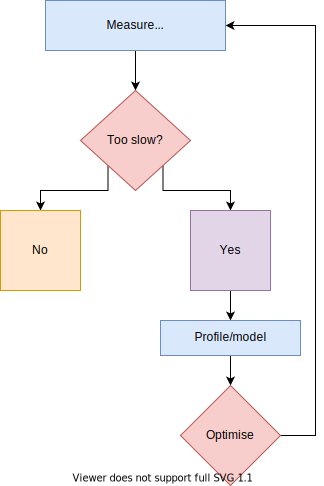
\includegraphics[height=0.8\textheight]{figures/optimisationworkflow}
  \end{center}
\end{frame}

\begin{frame}[fragile]
  \frametitle{Simple model for loop heavy code}
  \begin{columns}
    \begin{column}{0.4\textwidth}
      Simple view of hardware
      \begin{center}
        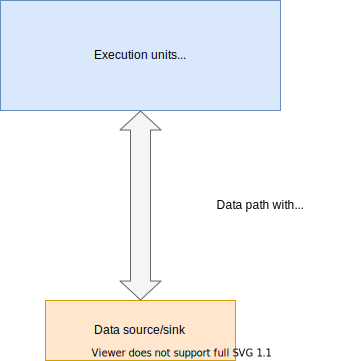
\includegraphics[width=\textwidth]{figures/rooflinecpumodel}
      \end{center}
    \end{column}
    \begin{column}{0.5\textwidth}
      Simple view of software

\begin{minted}{c}
/* Possibly nested loops */
for (i = 0; i < ...; i++)
 /* Complicated code doing */
 /* N FLOPs causing
 /* B bytes of data transfer */
\end{minted}

      Computational intensity [FLOPs/byte]
      \begin{equation*}
        I_c = \frac{N}{B}
      \end{equation*}
    \end{column}
  \end{columns}
\end{frame}

\begin{frame}
  \frametitle{Roofline}
  \begin{challenge}{What is the performance $P$ of a code?}
    How fast can work be done? $P$ measured in FLOPs/s
  \end{challenge}
  \begin{answer}{Bottleneck}
    Either
    \begin{itemize}
    \item execution of work $P_{\text{peak}}$ [FLOPs/s];
    \item or the data path $I_c b_s$ [FLOPs/byte $\times$ byte/s].
    \end{itemize}
    \begin{equation*}
      P = \min{(P_\text{peak}, I_c b_s)}
    \end{equation*}
  \end{answer}

  This is the simplest form of the roofline model. It is
  \emph{optimistic}, everything happens at ``light speed''.

  Introduced in Williams et al.~\emph{Roofline: An Insightful Visual
    Performance Model for Multicore Architectures}, CACM (2009).
  \url{https://doi.org/10.1145/1498765.1498785}
\end{frame}

\begin{frame}
  \frametitle{Roofline}
  \begin{center}
    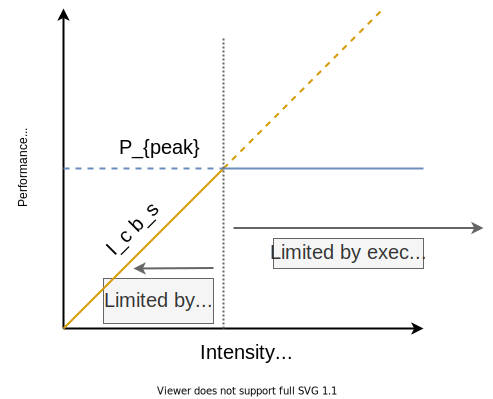
\includegraphics[height=0.8\textheight]{figures/rooflinesketch}
  \end{center}
\end{frame}

\begin{frame}
  \frametitle{Applying roofline}
  \begin{challenge}{Performance model}
    Roofline  characterises performance using three numbers:
    \begin{enumerate}
    \item $P_\text{peak}$ the peak floating point performance;
    \item $b_s$ the streaming memory bandwidth;
    \item $I_c$ the computational (or arithmetic) intensity of the code.
    \end{enumerate}

    The first two are characteristics of \emph{the hardware}. The last
    is a characteristic of the \emph{code}.
  \end{challenge}
  \begin{answer}{Idea}
    Measure these numbers and plot, gives idea of what performance
    optimisations are likely to pay off.
  \end{answer}
\end{frame}

\begin{frame}
  \frametitle{Example}
  \begin{center}
    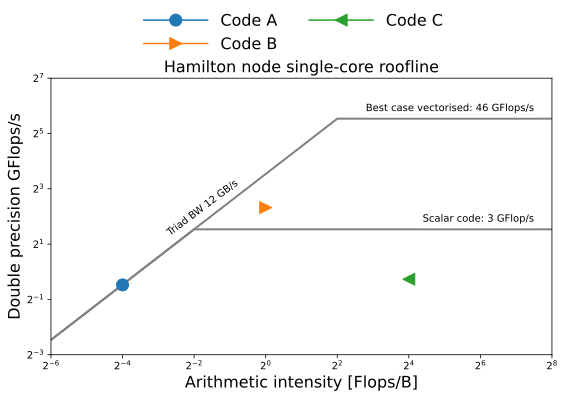
\includegraphics[height=0.8\textheight]{figures/roofline-example-simple}
  \end{center}
\end{frame}

\begin{frame}
  \frametitle{Guides optimisation choices}
  \begin{columns}
    \begin{column}{0.45\textwidth}
      \begin{center}
        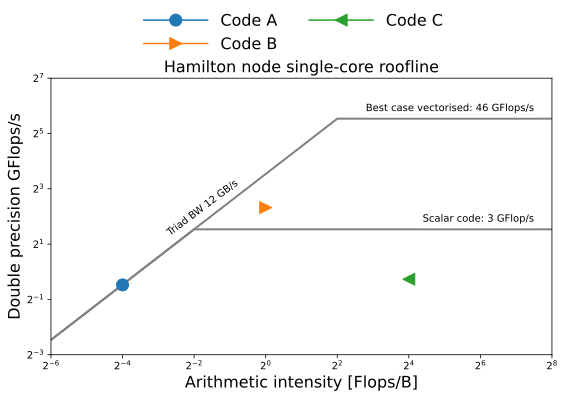
\includegraphics[width=\textwidth]{figures/roofline-example-simple}
      \end{center}
    \end{column}
    \begin{column}{0.45\textwidth}
      Which codes might benefit from vectorisation?

      How much improvement could we expect?

      Which codes might benefit from refactoring to increase
      arithmetic intensity?
    \end{column}
  \end{columns}
\end{frame}

\begin{frame}
  \frametitle{Determining machine characteristics}
  \begin{exampleblock}{Memory bandwidth}
    Roofline models data movement with streaming memory bandwidth.

    Two ways of computing it.
    \begin{enumerate}
    \item Know what speed of memory you have, and look up number of
      memory channels on spec sheet. For example, 4-channel 2.4GHz
      RAM delivers at best $4 \times 2.4\text{GHz} \times 8\text{Byte}
      = 76.8\text{GByte/s}$.\\
      $\Rightarrow$ Needs knowledge of installed memory,
      typically not achieved in practice. 
    \item \emph{Measure} using STREAM.\\
      $\Rightarrow$ we will typically do this (see exercise 4).
    \end{enumerate}
  \end{exampleblock}
\end{frame}

\begin{frame}
  \frametitle{Determining machine characteristics}
  \begin{exampleblock}{Floating point throughput}
    Absolute peak can be determined from spec sheet frequency and some
    knowledge of hardware.

    \begin{columns}
      \begin{column}{0.35\textwidth}
        \begin{center}
          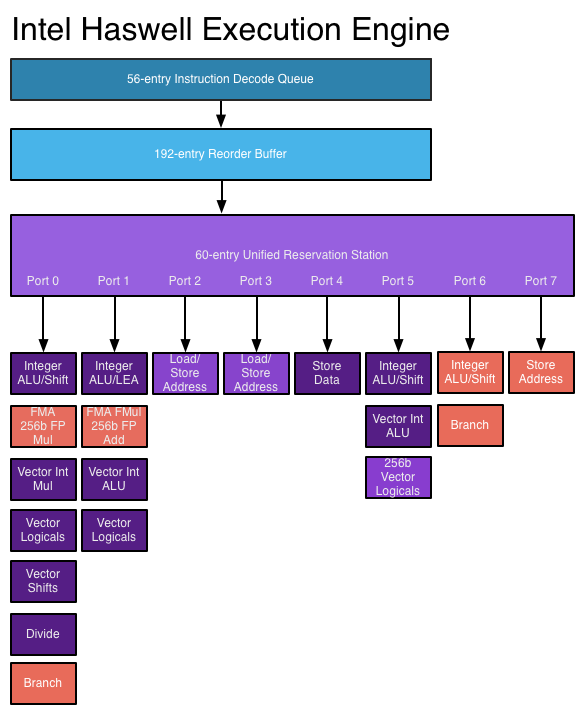
\includegraphics[width=\textwidth]{figures/haswellexec}
        \end{center}
      \end{column}
      \begin{column}{0.55\textwidth}
        \begin{itemize}
        \item Floating point instructions execute on port 0 and port 1
        \item Up to 4 ``micro-ops'' issued per cycle $\Rightarrow$ up
          to 2 floating point instructions per cycle
        \item FMA ($y \gets a + b\times c$); MUL execute on
          both ports.
        \item ADD only executes on port 1. Divide only executes on
          port 0.
        \end{itemize}
      \end{column}
    \end{columns}
  \end{exampleblock}
\end{frame}

\begin{frame}
  \frametitle{Determining machine characteristics}
  \begin{exampleblock}{Example: best case}
    Code only contains double precision SIMD FMAs, clock speed is 2.9GHz.

    Peak floating point throughput is

    \begin{equation*}
      \overbrace{2.9}^{\text{clock speed}} \times \underbrace{2}_{\text{dual issue}} \times
     \overbrace{4}^{\text{vector width}} \times \underbrace{2}_{\text{FMA}} = 46.4\text{GFLOPs/s} 
    \end{equation*}
  \end{exampleblock}
  \begin{exampleblock}{Example: only ADDs}
    Code only does double precision SIMD ADDs, clock speed is 2.9GHz.

    \begin{equation*}
      \overbrace{2.9}^{\text{clock speed}} \times \underbrace{1}_{\text{single issue}} \times
     \overbrace{4}^{\text{vector width}} = 11.6\text{GFLOPs/s} 
    \end{equation*}
  \end{exampleblock}
\end{frame}

\begin{frame}
  \frametitle{Determining machine characteristics}
  \begin{itemize}
  \item Often useful to put multiple ``roofs'' on the roofline,
    corresponding to different instruction mixes.
  \item Calculations are complicated by frequency scaling as well.
  \item[$\Rightarrow$] can add measured limit by running LINPACK (see exercises)
  \end{itemize}
  \begin{answer}{More details}
    \url{https://uops.info} has all the information you could ever
    want on micro-op execution throughput.

    \url{https://travisdowns.github.io/blog/2019/06/11/speed-limits.html}
    discusses in much more detail how to find limiting factors in
    (simple) code.
  \end{answer}
\end{frame}

\begin{frame}
  \frametitle{Computing arithmetic intensity}
  Two options:

  \begin{enumerate}
  \item Measure using performance counters (see later);
  \item Read code, count floating point operations and data accesses.
  \end{enumerate}

  Both options have their pros and cons.
\end{frame}
\begin{frame}[fragile]
  \frametitle{Counting operations}
\begin{minted}{c}
double *a, *b, *c, *d;
...
for (i = 0; i < N; i++) {
  a[i] = b[i]*c[i] + d[i]*a[i];
}
\end{minted}

  3 DP FLOPs/iteration. $3N$ total DP FLOPs. (Notice how we don't care about
  what type of FLOPs these are).
\end{frame}

\begin{frame}[fragile]
  \frametitle{Counting data accesses}
  Each read counts as one access. Each write counts as two (one load,
  one store). Only care about array data (ignore loop variables)
\begin{minted}{c}
double *a, *b, *c, *d;
...
for (i = 0; i < N; i++) {
  a[i] = b[i]*c[i] + d[i]*a[i];
}
\end{minted}

  3 DP reads, 1 DP write per iteration. $8\times 5N$ total bytes.
\end{frame}

\begin{frame}[fragile]
  \frametitle{Complication}
\begin{minted}{c}
double *a, *b, *c, *d;
for (i = 0; i < N; i++)
  for (j = 0; j < M; j++)
    a[j] = b[i]*c[i] + d[i]*a[j];
\end{minted}
  For actual data moved, need a \emph{model} of cache.
  \begin{answer}{Bounds on movement}
    \vspace{0.5\baselineskip}
    \begin{columns}[t]
      \begin{column}{0.45\textwidth}
        \begin{exampleblock}{Perfect cache}
          Provides lower bound.

          Each array entry moved from main memory once.

          Counts \emph{unique} memory accesses.

          $8\times 2M + 8\times 3N$ total bytes.
        \end{exampleblock}
      \end{column}
      \begin{column}{0.45\textwidth}
        \begin{challenge}{Pessimal cache}
          Provides upper bound

          Each array access misses cache.

          Counts \emph{total non-unique} memory accesses.

          $8 \times 2MN + 8\times 3MN$ total bytes.
        \end{challenge}
      \end{column}
    \end{columns}
  \end{answer}
\end{frame}

\begin{frame}
  \frametitle{Complication}
  \begin{answer}{Bounds on movement}
    \vspace{0.5\baselineskip}
    \begin{columns}[t]
      \begin{column}{0.45\textwidth}
        \begin{exampleblock}{Perfect cache}
          Provides lower bound.

          Each array entry moved from main memory once.

          Counts \emph{unique} memory accesses.

          $8\times 2M + 8\times 3N$ total bytes.
        \end{exampleblock}
      \end{column}
      \begin{column}{0.45\textwidth}
        \begin{challenge}{Pessimal cache}
          Provides upper bound

          Each array access misses cache.

          Counts \emph{total non-unique} memory accesses.

          $8 \times 2MN + 8\times 3MN$ total bytes.
        \end{challenge}
      \end{column}
    \end{columns}
  \end{answer}

  These bounds are typically not tight. If you want better bounds
  normally have to work harder in the analysis.

  Best employed in combination with measurement of arithmetic intensity.
\end{frame}
\begin{frame}
  \frametitle{Exercise: roofline plot for dense matrix-vector multiplication}
  \begin{itemize}
  \item Goal is to produce a roofline plot for dense matrix-vector
    multiplication, which computes

    \begin{equation*}
      \vec{y} = A \vec{x} = \sum_{j} A_{ij} \vec{x}_j
    \end{equation*}
  \end{itemize}
  \begin{center}
    \url{teaching.wence.uk/comp52315/exercises/exercise04/}
  \end{center}
\end{frame}
\end{document}
